\documentclass[12pt]{article}
\usepackage{amsmath}
\usepackage{amssymb}
\usepackage{cancel}
\usepackage{esdiff}
\usepackage{graphicx}
% \usepackage{physics}
\usepackage{siunitx}
\usepackage{wrapfig}

% \AtBeginDocument{\RenewCommandCopy\qty\SI}

\newcommand{\e}[1]{{\rm e}^{i\left( #1 \right)}}
\newcommand{\E}[1]{\times 10^{#1}}

\title{
    Chapter 16 End-of-Chapter Problems
    \\ \small
    Halliday \& Resnick, 10th Edition
}

\author{Donald Aingworth IV}

\date{\small Hit me where it Matters}

\begin{document}
    \DeclareSIUnit{\atm}{atm}
    \DeclareSIUnit{\cal}{\ cal}
    \DeclareSIUnit{\Cal}{\ Cal}
    \DeclareSIUnit{\calorie}{\ cal}
    \DeclareSIUnit{\Calorie}{\ Cal}
    \DeclareSIUnit{\celsiusdegree}{C^\circ}
    \DeclareSIUnit{\fahrenheit}{^\circ F}
    \DeclareSIUnit{\fahrenheitdegree}{F^\circ}
    \DeclareSIUnit{\torr}{\ torr}

    \maketitle

    \pagebreak
    \section{Problem 1}
        If a wave $y(x, t) = (6.0 \unit{\milli\meter}) \sin(kx + (600\,\unit{\radian/\second})t + \phi)$ travels along a string, how much time does any given point on the string take to move between displacements y = +2.0 mm and y = -2.0 mm?

        \subsection{Solution}
            Notice that the amplitude of the string is 6.0\unit{\milli\meter}. 
            Our positve and negative final amplitudes of y are 2 and -2 millimeters respectively.
            Note that these two values have a magnitude of one third of the amplitude.
            There are four points on the unit circle where the sine of the angle is $\frac{1}{3}$. 
            We can assume that the problem is asking the minumum time, since there are two ways that a point can travel between 2mm and -2mm.
            These two points would be for $kx + (600\,\unit{\radian/\second})t + \phi = \theta$, starting when $\theta = \arcsin\left( \frac{1}{3} \right)$ and ending when $\theta = \pi - \arcsin\left( \frac{1}{3} \right)$. 
            We can find the difference between these two. 
            \begin{align}
                \Delta \theta   &=  \theta_f - \theta_i
                    =   \pi - \arcsin\left( \frac{1}{3} \right) - \arcsin\left( \frac{1}{3} \right)\\
                    &=  2.462\,\unit{\radian}
            \end{align}

            As far as we consider it, the only thing in $kx + (600\,\unit{\radian/\second})t + \phi$ changing is $t$.
            Since we're generalizing, the other things besides $(600\,\unit{\radian/\second})t$ can be considered constants and initial conditons, so we can look at $t$.
            \begin{gather}
                \begin{align}
                    \Delta \theta &=    (kx + (600\,\unit{\radian/\second})t_f + \phi) - (kx + (600\,\unit{\radian/\second})t_i + \phi)\\
                        &=  (600\,\unit{\radian/\second}) (t_f - t_i)
                \end{align}\\
                \Delta t    =   \frac{\Delta \theta}{(600\,\unit{\radian/\second})}
                    =   \frac{2.462\,\unit{\radian}}{(600\,\unit{\radian/\second})}
                    =   \boxed{0.0041\,\unit{\second}}
            \end{gather}

            Note: if you were to find the minimum time between -2mm and 2mm, that would result in 1.1ms, but that is not the question posed here. 

    \pagebreak
    \section{Problem 3}
        A wave has an angular frequency of 110 rad/s and a wavelength of 1.80 m. 
        Calculate (a) the angular wave number and (b) the speed of the wave.

        \subsection{Solution (a)}
            We know the wavelength of the wave, which we can use to find the wave number.
            \begin{equation}
                k   =   \frac{2\pi}{\lambda}
                    =   \frac{2\pi}{1.80}
                    =   \frac{\pi}{0.9}
                    =   \boxed{3.49\,\unit{\radian/\meter}}
            \end{equation}

        \subsection{Solution (b)}
            We can use our angular wave number we found and the angular velocity to find the wave velocity.
            \begin{equation}
                v   =   \frac{\omega}{k}
                    =   \frac{110\,\unit{\radian/\second}}{\pi\,\unit{\radian}/0.9\,\unit{\meter}}
                    =   \frac{110 * 0.9}{\pi}\,\unit{\meter/\second}
                    =   \boxed{31.51\,\unit{\meter/\second}}
            \end{equation}

    \pagebreak
    \section{Problem 5}
        A sinusoidal wave travels along a string. 
        The time for a particular point to move from maximum displacement to zero is 0.170 s.
        What are the (a) period and (b) frequency? 
        (c) The wavelength is 1.40 m; what is the wave speed?

        \subsection{Solution (a)}
            The time to return from maximum displacement in one direction would be a quarter of the time to move from maximum displacement in the same direction (one period). 
            \begin{equation}
                T   =   4\,\Delta t
                    =   4 * 0.170\,\unit{\second}
                    =   \boxed{0.680\,\unit{\second}}
            \end{equation}

        \subsection{Solution (b)}
            The frequency is the reciprocal of the period. 
            \begin{equation}
                f   =   \frac{1}{T}
                    =   \frac{1}{0.680\,\unit{\second}}
                    =   \boxed{1.47\,\unit{\hertz}}
            \end{equation}

        \subsection{Solution (c)}
            The velocity is equal to the wavelength divided by the period.
            \begin{equation}
                v   =   \frac{\lambda}{T}
                    =   \frac{1.40\,\unit{\meter}}{0.680\,\unit{\second}}
                    =   \boxed{2.06\,\unit{\meter/\second}}
            \end{equation}

    \pagebreak
    \section{Problem 9}
        \begin{wrapfigure}{r}{0.25\textwidth}
            \vspace{-30pt}
            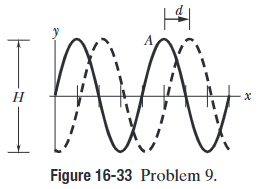
\includegraphics[width=0.25\textwidth]{picture_16-33.png} 
            % \label{fig:wrapfig}
        \end{wrapfigure}
        A sinusoidal wave moving along a string is shown twice in Fig. 16-33, as crest A travels in the positive direction of an x axis by distance d = 6.0 cm in 4.0 ms. 
        The tick marks along the axis are separated by 10 cm; height H = 6.00 mm.
        The equation for the wave is in the form $y(x, t) = y_m \sin(kx \pm \omega t)$, so what are (a) $y_m$, (b) $k$, (c) $\omega$, and (d) the correct choice of sign in front of $\omega$?

        \subsection{Solution}
            The velocity of the wave would be equivalent to the distance covered divided by the time taken.
            \begin{equation}
                v   =   \frac{\Delta x}{\Delta t}
                    =   \frac{0.06\,\unit{\meter}}{0.004\,\unit{\second}}
                    =   15\,\unit{\meter/\second}
            \end{equation}

            The amplitude would also be equal to half the distance between the top and bottom peaks ($H$).
            \begin{equation}
                A   =   \frac{H}{2}
                    =   \frac{6\,\unit{\milli\meter}}{2}
                    =   3\,\unit{\milli\meter}
                    =   y_m
            \end{equation}

            Note that the wave goes through one period over the course of four tick marks of a length of 10 \unit{\centi\meter} each, equivalent to 40 \unit{\centi\meter} total. 
            This would be equivalent to the wavelength, which can be used to find the frequency.
            This frequency cna be used to find the angular velocity.
            \begin{gather}
                v   =   \lambda f \to
                f   =   \frac{v}{\lambda}
                    =   \frac{15\,\unit{\meter/\second}}{0.4\,\unit{\meter}}
                    =   37.5\,\unit{\hertz}\\
                f   =   \frac{\omega}{2\pi} \to
                \omega  =   2\pi f
                    =   75\pi\,\unit{\radian/\second}
            \end{gather}

            Knowing our velocity and engular velocity, we can use this to find the angular wave number.
            \begin{gather}
                v   =   \frac{\omega}{k} \to
                k   =   \frac{\omega}{v}
                    =   \frac{75\pi\,\unit{\radian/\second}}{15\,\unit{\meter/\second}}
                    =   5\pi\,\unit{\radian/\meter}
            \end{gather}

            We have our values needed to fill out the sinusoidal wave.
            Since the wave travels in a positive direction, the sign here would be negative.
            \begin{equation}
                \boxed{y(x,t) = (3\,\unit{\milli\meter})\sin((5\pi\,\unit{\radian/\meter})x - (75\pi\,\unit{\radian/\second})t)}
            \end{equation}

    % \pagebreak
    \section{Problem 15}
        A stretched string has a mass per unit length of 5.00 g/cm and a tension of 10.0 N. 
        A sinusoidal wave on this string has an amplitude of 0.12 mm and a frequency of 100 Hz and is traveling in the negative direction of an x axis. 
        If the wave equation is of the form $y(x, t) = y_m \sin(kx \pm \omega t)$, what are (a) $y_m$, (b) $k$, (c) $\omega$, and (d) the correct choice of sign in front of $\omega$?

        \subsection{Solution}
            We have the value of the amplitude, whch would be equal to $y_m$.
            \begin{equation}
                y_m =   A
                    =   0.12\,\unit{\milli\meter}
            \end{equation}

            Our frequency can give us the value of $\omega$.
            \begin{gather}
                f   =   \frac{\omega}{2\pi}\\
                \omega  =   2\pi f
                    =   2\pi * 100\,\unit{\hertz}
                    =   200\pi\,\unit{\radian/\second}
            \end{gather} 

            For the wave number $k$, we can start by finding the speed of the wave.
            This should be done under consideration of a stretched string.
            \begin{gather}
                v   =   \sqrt{\frac{\tau}{\mu}}
                    =   \sqrt{\frac{10.0\,\unit{\newton}}{5.00\,\unit{\gram/\centi\meter}}}
                    =   \sqrt{\frac{100.0\,\unit{\newton}}{5.00\unit{\kilo\gram/\meter}}}
                    =   \sqrt{20\,\unit{\meter^2/\second^2}}
            \end{gather}

            This in turn can be used in conjuction with the angular velocity of the wave. 
            \begin{gather}
                v   =   \frac{\omega}{k}\\
                k   =   \frac{\omega}{v}
                    =   \frac{200\pi\,\unit{\radian/\second}}{\sqrt{20\,\unit{\meter^2/\second^2}}}
                    =   140.5\,\unit{\meter^{-1}}
            \end{gather}

            Since the wave is traveling in the negative direction, the sign would be positive.
            \begin{equation}
                \boxed{y(x,t)   =   (1.2\E{-4}\,\unit{\meter})\sin((140.5\,\unit{\meter^{-1}})x + (200\pi\,\unit{\radian/\second})t)}
            \end{equation}

    \pagebreak
    \section{Problem 19}
        What is the speed of a transverse wave in a rope of length 2.00 m and mass 60.0 g under a tension of 500 N?

        \subsection{Solution}
            First find the linear density of the rope.
            \begin{equation}
                \mu =   \frac{m}{L}
                    =   \frac{0.060\,\unit{\kilo\gram}}{2.00\,\unit{\meter}}
                    =   0.03\,\unit{\kilo\gram/\meter}
            \end{equation}
            Then, use the formula for the speed of the wave. 
            \begin{equation}
                v   =   \sqrt{\frac{\tau}{\mu}}
                    =   \sqrt{\frac{500\,\unit{\newton}}{0.03\,\unit{\kilo\gram/\meter}}}
                    =   \boxed{129.1\,\unit{\meter/\second}}
            \end{equation}

    \pagebreak
    \section{Problem 21}
        A 100 g wire is held under a tension of 250 N with one end at $x = 0$ and the other at $x = 10.0$ m. 
        At time $t = 0$, pulse 1 is sent along the wire from the end at $x = 10.0$ m. 
        At time $t = 30.0$ ms, pulse 2 is sent along the wire from the end at $x = 0$. 
        At what position $x$ do the pulses begin to meet?

        \subsection{Solution}
            Since the wire is a wire, the speed can be calculated by first finding the linear density and then the wave velocity. 
            \begin{gather}
                \mu =   \frac{m}{L}
                    =   \frac{0.1\,\unit{\kilo\gram}}{10.0\,\unit{\meter}}
                    =   0.01\,\unit{\kilo\gram/\meter}\\
                v   =   \sqrt{\frac{\tau}{\mu}}
                    =   \sqrt{\frac{250\,\unit{\newton}}{0.01\,\unit{\kilo\gram/\meter}}}
                    =   \sqrt{25000\,\unit{\meter^2/\second^2}}
                    =   50\,\sqrt{10}\,\unit{\meter/\second}
            \end{gather}

            This will be the speed of both waves, which we can use to find the location of the first wave when the second wave starts up.
            \begin{align}
                \Delta x    &=  v * \Delta t
                    =   50\,\sqrt{10}\,\unit{\meter/\second} \times 30\E{-3}\,\unit{\second}
                    =   1.5\,\sqrt{10}\,\unit{\meter}\\
                x_i &=  L - \Delta x
                    =   10.0\,\unit{\meter} - 1.5\,\sqrt{10}\,\unit{\meter}
                    =   \frac{20 - 3\sqrt{10}}{2}\,\unit{\meter}
            \end{align}

            Since the waves will be traveling at the same speed in opposite directions, they will meet at the average point of their starting points. 
            \begin{align}
                x_{\rm avg} &=  \frac{x_i}{2}
                    =   \frac{20 - 3\sqrt{10}}{4}\,\unit{\meter}
                    =   \boxed{2.628\,\unit{\meter}}
            \end{align}

    \pagebreak
    \section{Problem 25}
        A uniform rope of mass $m$ and length $L$ hangs from a ceiling. 
        (a) Show that the speed of a transverse wave on the rope is a function of $y$, the distance from the lower end, and is given by $v = \sqrt{gy}$.
        (b) Show that the time a transverse wave takes to travel the length of the rope is given by $t = 2\sqrt{L/g}$.

        \subsection{Solution (a)}
            There are two deterministic factors for the velocity of the wave: the tension force and the density of the wire. 
            There are equations for each of these and they can be put into the velocity equation.
            The tension force would be equal to the downward force on the portion of the wire, which would only be the gravitational force.
            \begin{gather}
                \tau    =   F_g
                    =   mg * \frac{y}{L}\\
                \mu =   \frac{m}{L}\\
                v   =   \sqrt{\frac{mg}{m/L} * \frac{y}{L}}
                    =   \sqrt{gy}
            \end{gather}

        \subsection{Solution (b)}
            The formula for time taken at a specific speed can be calculated by dividing the distance by the speed.
            \begin{gather}
                t   =   \frac{\Delta x}{v}
                    =   \frac{dx}{\sqrt{gy}}
            \end{gather}

            Since the velocity is dependant on the y-position, we can find the total time by integrating over $y$. 
            \begin{align}
                t   &=  \int_{0}^{L}\frac{1}{\sqrt{gy}}\,dy
                    =   2\frac{\sqrt{y}}{\sqrt{g}}\,dy
                    =   2\sqrt{L/g}
            \end{align}

    \pagebreak
    \section{Problem 30}
        Use the wave equation to find the speed of a wave given in terms of the general function $h(x, t)$:
        \begin{equation}
            y(x, t) = (4.00 \unit{\milli\meter}) h[(30 \unit{\meter^{-1}})x + (6.0\,\unit{\second^{-1}})t]
        \end{equation}

        \subsection{Solution}
            We can just take the second derivative of $y(x,t)$ with regard to both $x$ and $t$.
            Let's start with $x$.
            \begin{align}
                y(x,t)  &=  (4.00 \unit{\milli\meter}) h[(30 \unit{\meter^{-1}})x + (6.0\,\unit{\second^{-1}})t]\\
                \diff{y}{x}    &=  (30\,\unit{\meter^{-1}}) (4.00 \unit{\milli\meter}) h'[(30 \unit{\meter^{-1}})x + (6.0\,\unit{\second^{-1}})t]\\
                \diff[2]{y}{x} &=  (30\,\unit{\meter^{-1}})^2 (4.00 \unit{\milli\meter}) h''[(30 \unit{\meter^{-1}})x + (6.0\,\unit{\second^{-1}})t]
            \end{align}

            Now we can do with respect to $t$.
            \begin{align}
                y(x,t)  &=  (4.00 \unit{\milli\meter}) h[(30 \unit{\meter^{-1}})x + (6.0\,\unit{\second^{-1}})t]\\
                \diff{y}{t}    &=  (6.0\,\unit{\second^{-1}}) (4.00 \unit{\milli\meter}) h'[(30 \unit{\meter^{-1}})x + (6.0\,\unit{\second^{-1}})t]\\
                \diff[2]{y}{t}  &=  (6.0\,\unit{\second^{-1}})^2 (4.00 \unit{\milli\meter}) h''[(30 \unit{\meter^{-1}})x + (6.0\,\unit{\second^{-1}})t]
            \end{align}

            Now we can substitute both of them into the wave equation.
            \begin{equation}
                \diffp[2]{\psi}{x}  =   \frac{1}{v^2} \diffp[2]{\psi}{t}
            \end{equation}

            Noticing that within our earlier second derivatives, there is the identical component of $(4.00 \unit{\milli\meter}) h''[(30 \unit{\meter^{-1}})x + (6.0\,\unit{\second^{-1}})t]$, which we can preemptively cancel out on both sides.
            \begin{gather}
                (30\,\unit{\meter^{-1}})^2  =   \frac{1}{v^2}\,(6.0\,\unit{\second^{-1}})^2\\
                \frac{(6.0\,\unit{\second})^2}{(30\,\unit{\meter})^2}   =   \frac{1}{v^2}\\
                v^2 =   \frac{(30\,\unit{\meter})^2}{(6.0\,\unit{\second})^2}\\
                v   =   \frac{30\,\unit{\meter}}{6\,\unit{\second}}
                    =   \boxed{5.0\,\unit{\meter/\second}}
            \end{gather}

    \pagebreak
    \section{Problem 31}
        Two identical traveling waves, moving in the same direction, are out of phase by $\pi/2$ rad. 
        What is the amplitude of the resultant wave in terms of the common amplitude $y_m$ of the two combining waves?

        \subsection{Solution}
        We can set equations for both waves.
        I will be using complex notation, since I prefer it that way.
        \begin{align}
            \Psi_1(x,t) &=  y_m \e{kx - \omega t}\\
            \Psi_2(x,t) &=  y_m \e{kx - \omega t + \frac{\pi}{2}}\\
            \Psi(x,t)   &=  \Psi_1(x,t) + \Psi_2(x,t)
                =   y_m \e{kx - \omega t} + y_m \e{kx - \omega t + \frac{\pi}{2}}\\
                &=  y_m \e{kx - \omega t}\left( 1 + e^{i\frac{\pi}{2}} \right)
                =   y_m \e{kx - \omega t}\left( 1 + i \right)\\
                &=  y_m \e{kx - \omega t} * \sqrt{2}\e{\pi/2}
                =   y_m \sqrt{2} \e{kx - \omega t + \frac{\pi}{2}}
        \end{align}

        This gives another wave form equation. 
        It gives our wave an amplitude. 
        \begin{equation}
            A   =   y_m \sqrt{2}
                =   \boxed{1.414 y_m}
        \end{equation}

    \pagebreak
    \section{Problem 35}
        Two sinusoidal waves of the same frequency travel in the same direction along a string. 
        If $y_{m1} = 3.0 \unit{\centi\meter}$, $y_{m2} = 4.0 \unit{\centi\meter}$, $\phi_1 = 0$, and $\phi_2 = \pi/2$ rad, what is the amplitude of the resultant wave?

        \subsection{Solution}
            Since they have the same frequency, they have the same angular speed.
            \begin{align}
                \Psi_1  &=  y_{m1}\e{kx - \omega t + \phi_1}
                    =   (3.0 \unit{\centi\meter})\e{kx - \omega t + 0}\\
                \Psi_2  &=  y_{m2}\e{kx - \omega t + \phi_2}
                    =   (4.0 \unit{\centi\meter})\e{kx - \omega t + \frac{\pi}{2}}\\
                \Psi    &=  \Psi_1 + \Psi_2
                    =   (3.0 \unit{\centi\meter})\e{kx - \omega t + 0} + (4.0 \unit{\centi\meter})\e{kx - \omega t + \frac{\pi}{2}}\\
                    &=  \e{kx - \omega t} \left( (3.0 \unit{\centi\meter}) + (4.0 \unit{\centi\meter})\e{\frac{\pi}{2}} \right)\\
                    &=  \e{kx - \omega t} \left( 3.0 \unit{\centi\meter} + 4.0i \unit{\centi\meter} \right)
            \end{align}

            This associates well wth a 3-4-5 triangle.
            We know that triangle has an hypotenuse of length 5cm can designate that that triangle has an angle of $\theta$.
            \begin{align}
                \Psi    &=  \e{kx - \omega t} * (5\unit{\centi\meter})\e{\theta}
                    =   (5 \unit{\centi\meter})\e{kx - \omega t + \theta}\\
                A   &=  \boxed{5\,\unit{\centi\meter}}
            \end{align}

    \pagebreak
    \section{Problem 37}
        These two waves travel along the same string:
        \begin{align}
            y_1(x, t)   &=  (4.60 \unit{\milli\meter}) \sin(2\pi x - 400\pi t)\\
            y_2(x, t)   &=  (5.60 \unit{\milli\meter}) \sin(2\pi x - 400\pi t + 0.80\pi\,\unit{\radian}).
        \end{align}
        What are (a) the amplitude and (b) the phase angle (relative to wave 1) of the resultant wave? 
        (c) If a third wave of amplitude 5.00 mm is also to be sent along the string in the same direction as the first two waves, what should be its phase angle in order to maximize the amplitude of the new resultant wave?

        \subsection{Solution (a)}
            I'll start by turning the two waves complex.
            This is entirely optional.
            \begin{align}
                y_1(x, t)   &=  (4.60 \unit{\milli\meter})i \e{2\pi x - 400\pi t}\\
                y_2(x, t)   &=  (5.60 \unit{\milli\meter})i \e{2\pi x - 400\pi t + 0.80\pi\,\unit{\radian}}
            \end{align}

            Now we add them together.
            \begin{align}
                \Psi(x,t)   &=  y_1(x, t) + y_2(x, t)\\
                    &=  (4.60 \unit{\milli\meter})i \e{2\pi x - 400\pi t} + (5.60 \unit{\milli\meter})i \e{2\pi x - 400\pi t + 0.80\pi\,\unit{\radian}}\\
                    &=  i \e{2\pi x - 400\pi t} (4.60 \unit{\milli\meter} + 5.60 \unit{\milli\meter}\,\e{0.80\pi\,\unit{\radian}})\\
                    &=  i \e{2\pi x - 400\pi t} (4.60\,\unit{\milli\meter} - 4.53\,\unit{\milli\meter} + 3.29i\,\unit{\milli\meter})\\
                    &=  i \e{2\pi x - 400\pi t} (0.07\,\unit{\milli\meter} + 3.29i\,\unit{\milli\meter})
            \end{align}

            From here, we can find the amplitude.
            \begin{align}
                A   &=  \sqrt{0.07^2 + 3.29^2}
                    =   \boxed{3.292\,\unit{\milli\meter}}
            \end{align}

        \subsection{Solution (b)}
            This can finally be used to find the phase angle.
            \begin{equation}
                \arctan\left( \frac{3.29}{0.07} \right) =   \boxed{1.55\,\unit{\radian}}
            \end{equation}

            It can be used to set up a final equation.
            \begin{align}
                \Psi(x,t)   &=  (3.292\,\unit{\milli\meter}) i \e{2\pi x - 400\pi t + 1.55}
            \end{align}

        \subsection{Solution (c)}
            Give it the same phase angle of \boxed{1.55\,\unit{\radian}}. 

    % \pagebreak
    \section{Problem 41}
        A string fixed at both ends is 8.40 m long and has a mass of 0.120 kg. 
        It is subjected to a tension of 96.0 N and set oscillating. 
        (a) What is the speed of the waves on the string? 
        (b) What is the longest possible wavelength for a standing wave? 
        (c) Give the frequency of that wave.

        \subsection{Solution (a)}
            First, take the formula for the linear density $\mu$.
            \begin{equation}
                \mu =   \frac{m}{\ell}
            \end{equation}

            Substitute that into the formula for the wave speed and solve.
            \begin{align}
                v   &=  \sqrt{\frac{\tau}{m/\ell}}
                    =   \sqrt{\frac{\tau \ell}{m}}
                    =   \sqrt{\frac{96.0\,\unit{\newton} * 8.40\,\unit{\meter}}{0.120\,\unit{\kilo\gram}}}\\
                    &=  \sqrt{\frac{806.4\,\unit{\joule}}{0.120\,\unit{\kilo\gram}}}
                    =   \sqrt{6720\,\unit{\meter^2/\second^2}}
                    =   \boxed{81.9756\,\unit{\meter/\second}}
            \end{align}

        \subsection{Solution (b)}
            The longest possible standing wave wavelength would be the length of the string itself.
            This would leave it with a wavelength of \boxed{8.40\,\unit{\meter}}. 

        \subsection{Solution (c)}
            The frequency is calculatable from the velocity and the wavelength.
            \begin{gather}
                v   =   \lambda f\\
                \begin{align}
                    f   &=  \frac{v}{\lambda}
                        =   \frac{81.9756\,\unit{\meter/\second}}{8.40\,\unit{\meter}}
                        =   \boxed{9.759\,\unit{\hertz}}
                \end{align}
            \end{gather}

    % \pagebreak
    \section{Problem 43}
        What are (a) the lowest frequency, (b) the second lowest frequency, and (c) the third lowest frequency for standing waves on a wire that is 10.0 m long, has a mass of 100 g, and is stretched under a tension of 250 N?

        \subsection{Solution (a)}
            First find the velocity.
            \begin{align}
                v   &=  \sqrt{\frac{\tau}{\mu}}
                    =   \sqrt{\frac{\tau}{m/L}}
                    =   \sqrt{\frac{250\,\unit{\newton} * 10.0\,\unit{\meter}}{0.1\,\unit{\kilo\gram}}}\\
                    &=  \sqrt{\frac{2500\,\unit{\newton\cdot\meter}}{0.1\,\unit{\kilo\gram}}}
                    =   \sqrt{25000\,\unit{\meter^2/\second^2}}
                    =   50\sqrt{10}\,\unit{\meter/\second}
            \end{align}

            The lowest speed would have a wavelength of twice the length of the wire.
            We can use this to find the frequency, using the equation $v = \lambda f$.
            \begin{align}
                f   &=  \frac{v}{\lambda}
                    =   \frac{50\sqrt{10}\,\unit{\meter/\second}}{20\,\unit{\meter}}
                    =   \boxed{2.5\sqrt{10}\,\unit{\hertz}}
            \end{align}

        \subsection{Solution (b)}
            In this case, the wavelength will be the length of the string.
            \begin{align}
                f   &=  \frac{v}{\lambda}
                    =   \frac{50\sqrt{10}\,\unit{\meter/\second}}{10\,\unit{\meter}}
                    =   \boxed{5\sqrt{10}\,\unit{\hertz}}
            \end{align}
            
        \subsection{Solution (c)}
            In this case, the wavelength will be two thirds the length of the string.
            \begin{align}
                f   &=  \frac{v}{\lambda}
                    =   \frac{50\sqrt{10}\,\unit{\meter/\second}}{\frac{2}{3}*10\,\unit{\meter}}
                    =   \boxed{7.5\sqrt{10}\,\unit{\hertz}}
            \end{align}

    \pagebreak
    \section{Problem 45}
        A string that is stretched between fixed supports separated by 75.0 cm has resonant frequencies of 420 and 315 Hz, with no intermediate resonant frequencies. 
        What are (a) the lowest resonant frequency and (b) the wave speed?

        \subsection{Solution (a)}
            There's an equation for the resonnant frequency.
            We can apply this ot the two cases.
            \begin{align}
                420\,\unit{\hertz}  &=  (n + 1)\frac{v}{2L}\\
                315\,\unit{\hertz}  &=  n\frac{v}{2L}
            \end{align}

            Subtract the latter from the former to find the lowest resonant frequency (i.e. n = 1).
            \begin{align}
                420\,\unit{\hertz} - 315\,\unit{\hertz} &=  \frac{v}{2L}
                    =   f_1
                    =   \boxed{105\,\unit{\hertz}}
            \end{align}

        \subsection{Solution (b)}
            To find the wave speed, we can use the resonant frequency at n = 1.
            \begin{gather}
                f   =   \frac{v}{2L}\\
                v   =   2fL
                    =   2 * 105\,\unit{\hertz} * 0.75\,\unit{\centi\meter}
                    =   \boxed{157.5\,\unit{\meter/\second}}
            \end{gather}

    \pagebreak
    \section{Problem 53}
        A string oscillates according to the equation
        \begin{equation}
            y = (0.50 \unit{\centi\meter}) \sin \left[  \left( \frac{\pi}{3}\,\unit{\centi\meter^{-1}} \right)x \right] \cos\left[ (40\pi\,\unit{\second^{-1}} )t \right]
        \end{equation}
        What are the (a) amplitude and (b) speed of the two waves (identical except for direction of travel) whose superposition gives this oscillation? 
        (c) What is the distance between nodes? 
        (d) What is the transverse speed of a particle of the string at the position x = 1.5 cm when t = $\frac{9}{8}$ s?

        \subsection{Solution (a)}
            If the two waves are identical, their amplitudes will be identical.
            The amplitude of each would be half the length of their combination.
            \begin{equation}
                \frac{5\,\unit{\milli\meter}}{2}    =   \boxed{2.5\,\unit{\milli\meter}}
            \end{equation}

        \subsection{Solution (b)}
            There's a 

    \pagebreak
    \section{Problem 61}

        \subsection{Solution}

    \pagebreak
    \section{Problem 65}

        \subsection{Solution}

    \pagebreak
    \section{Problem 73}

        \subsection{Solution}

    \pagebreak
    \section{Problem 75}

        \subsection{Solution}

    \pagebreak
    \section{Problem 83}

        \subsection{Solution}

    \pagebreak

    \tableofcontents
    
\end{document}